\documentclass[10pt]{article}
\usepackage{polski}
\usepackage[utf8]{inputenc}
\usepackage{amsmath}
\usepackage{amsfonts}
\usepackage{tabto,lipsum}
\usepackage{calc}
\usepackage{xcolor}
\usepackage{graphicx}
\graphicspath{ {./img/} }
\usepackage{shadowtext}
\usepackage{hyperref}
\hypersetup{%
  colorlinks=false,% hyperlinks will be black
  linkbordercolor=red,% hyperlink borders will be red
  pdfborderstyle={/S/U/W 1}% border style will be underline of width 1pt
}
\usepackage[margin=1.5cm]{geometry}
\usepackage{algpseudocode}
\usepackage{algorithm}
\usepackage{listings}
\usepackage{ulem}
\usepackage{cancel}
\usepackage{adjustbox}
\usepackage{pgfplots}

\PassOptionsToPackage{usenames,dvipsnames,svgnames}{xcolor}
\usepackage{tikz}
\usetikzlibrary{arrows,positioning,automata}

\linespread{1.3}

\title{Obliczenia Naukowe,\\Laboratorium, Lista 2}
\author{Jerzy Wroczyński}
\date{2020-11-08}

\begin{document}

\maketitle

\section{Zadanie 1.}

\subsection{Opis problemu}
Należy napisać program liczący iloczyn skalarny dwóch wektorów przy pomocy czterech metod w dwóch arytmetykach (\texttt{Float32} oraz \texttt{Float64}).

Zgodnie z poleceniem zadania wektor $x$ został nieco zmieniony.
$$
\begin{aligned}
    x &= [2.718281828, -3.141592654, 1.414213562, 0.577215664\boldmath\cancel{9}, 0.301029995\boldmath\cancel{7}]\\
    y &= [1486.2497, 878366.9879, -22.37492, 4773714.647, 0.000185049]
\end{aligned}
$$

\subsection{Rozwiązanie}

(kod źródłowy w pliku \texttt{ex-1.jl})

Aby uruchomić program, należy wykonać polecenie \texttt{./ex-1.jl} — wyświetlą się instrukcje mówiące, jakie argumenty są przyjmowane przez program.

Wyniki:
(l1 — wyniki z pierwszej listy; l2 — wyniki po zastosowanych zmianach wymienionych w poleceniu)
\begin{itemize}
    \item \texttt{Float32}
    \begin{itemize}
        \item metoda \textit{„w przód”}
        \begin{itemize}
            \item $= -0.2499443$ (l1)
            \item $= -0.2499443$ (l2)
        \end{itemize}
        \item metoda \textit{„w tył”}
        \begin{itemize}
            \item $= -0.2043457$ (l1)
            \item $= -0.2043457$ (l2)
        \end{itemize}
        \item od \textbf{największego} do \textit{najmniejszego}
        \begin{itemize}
            \item $= -0.25$ (l1)
            \item $= -0.25$ (l2)
        \end{itemize}
        \item od \textit{najmniejszego} do \textbf{największego}
        \begin{itemize}
            \item $= -0.25$ (l1)
            \item $= -0.25$ (l2)
        \end{itemize}
    \end{itemize}
    \item \texttt{Float64}
    \begin{itemize}
        \item metoda \textit{„w przód”}
        \begin{itemize}
            \item $= 1.0251881368296672 \cdot 10^{-10}$ (l1)
            \item $= -0.004296342739891585$ (l2)
        \end{itemize}
        \item metoda \textit{„w tył”}
        \begin{itemize}
            \item $= -1.5643308870494366 \cdot 10^{-10}$ (l1)
            \item $= -0.004296342998713953$ (l2)
        \end{itemize}
        \item od \textbf{największego} do \textit{najmniejszego}
        \begin{itemize}
            \item $= 0$ (l1)
            \item $= -0.004296342842280865$ (l2)
        \end{itemize}
        \item od \textit{najmniejszego} do \textbf{największego}
        \begin{itemize}
            \item $= 0$ (l1)
            \item $= -0.004296342842280865$ (l2)
        \end{itemize}
    \end{itemize}
\end{itemize}

Faktyczna wartość wynosi $-1.00657107000000 \cdot 10^{-11}$.

\textit{W przypadku arytmetyki \texttt{Float32} nie widać żadnych różnic (za mała precyzja), ale w przypadku \texttt{Float64} zachodzą bardzo zauważalne różnice. Problem jest w uwarunkowaniu zadania — wartości, które sumujemy mają różne znaki.}

\section{Zadanie 2.}

\subsection{Opis problemu}

Należy obliczyć granicę funkcji $f(x) = e^x \cdot \ln(1 + e^{-x})$ oraz narysować wykres tej funkcji przy pomocy dwóch różnych programów.

\subsection{Rozwiązanie}

Liczymy granicę
$$
e^x \cdot \ln(1 + e^{-x}) = \frac{\ln(1 + e^{-x})}{e^{-x}} \xrightarrow{\text{z zasady de l’Hôpitala}}
\frac{(ln(1 + e^{-x}))'}{(e^{-x})'} =
-\frac{1}{(e^x + 1) \cdot (-e^{-x})} =
\frac{1}{1 + e^{-x}} \xrightarrow[]{x \to \infty} 1
$$

\noindent Poniżej znajdują się dwa wykresy funkcji $f$.

\begin{figure}[H]
    \centering
    \def\svgwidth{0.8\columnwidth}
    \input{ex-2-1.pdf_tex}
    \caption{Wykres wykonany przy pomocy programu \textit{Wolfram Mathematica}}
\end{figure}

\begin{figure}[H]
    \centering
    \includegraphics{ex-2-2.png}
    \caption{Wykres wykonany przy pomocy \textit{Kalkulatora Google}}
\end{figure}

Przy wartościach $x$ około $30$ widać pewne anomalie. Funkcja zaczyna być coraz bardziej niestabilna, aż w końcu osiąga stałe zero (niezgodne z obliczoną wartością granicy). Funkcję $f$ możemy w zasadzie rozbić na dwie części — $g(x) = e^x$ oraz $h(x) = \ln(1 + e^{-x})$. Otóż funkcja $g$ dąży do nieskończoności, kiedy $h$ dąży do zera. Po obliczeniu granicy dochodzimy do wniosku, że te dwie funkcje się nawzajem \textit{anulują}. Przy czym to zjawisko \textit{nullifikacji} ma swoje \textit{granice} i właśnie w pewnym momencie niedokładna komputerowa symulacja liczb rzeczywistych nie jest w stanie dokładnie określić wartości funkcji $f$ dalej niż $x = 30$. Zbliżając się do okolic epsilona maszynowego w przypadku $e^{-x}$ powoduje brak precyzji.

\section{Zadanie 3.}

\subsection{Opis problemu}

Należy rozwiązać klasyczne zadanie z równaniem $Ax = b$ gdzie $x$ to jest po prostu kolumna jedynek — należy sprawdzić jak daleki jest $\tilde{x}$ od tego prawdziwego $x$.

Używamy tutaj dwóch sposobów obliczenia rozwiązania:
\begin{itemize}
    \item metoda Gaussa $\tilde{x} = \frac{b}{A}$ (\texttt{x = A\textbackslash b})
    \item metoda odwracania $\tilde{x} = A^{-1} \cdot b$ (\texttt{x = inv(A)*b})
\end{itemize}
gdzie macierz $A$ jest równa macierzy Hilberta $H_n$ (generujemy funkcją \texttt{hilb} z pliku \texttt{hilb.jl})
oraz losowej macierzy stopnia $n$ z zadanym wskaźnikiem uwarunkowania $c$ (generujemy funkcją \texttt{matcond} z pliku \texttt{matcond.jl}).

\subsection{Rozwiązanie}

W pliku \texttt{ex-3.jl} znajduje się program, który od razu wyświetla \texttt{rank} i \texttt{cond} macierzy oraz sam błąd względny $\frac{||x - \tilde{x}||}{||x||}$ (sam $\tilde{x}$ nie jest tutaj istotny — to właśnie odchylenie daje nam lepszy obraz eksperymentu).

Uruchamiając program \texttt{./ex-3.jl}, otrzymujemy wyniki:

$H_n$:
\begin{center}
    \begin{tabular}{|c| c c c c|}
        \hline
        n & $\operatorname{cond}(A)$ & $\operatorname{rank}(A)$ & błąd wzgl. dla metody Gaussa & błąd wzgl. dla metody odwracania\\
        \hline\hline
        2 & 19.28147006790397 & 2 & 5.661048867003676e-16 & 1.4043333874306803e-15\\
        3 & 524.0567775860644 & 3 & 8.022593772267726e-15 & 0.0\\
        4 & 15513.738738928929 & 4 & 4.637277712035294e-13 & 7.542470546988852e-13\\
        5 & 476607.25024224253 & 5 & 1.7697056701418277e-13 & 7.45602798259539e-12\\
        6 & 1.495105864125091e7 & 6 & 3.496491467713994e-10 & 3.533151828962887e-10\\
        7 & 4.7536735637688667e8 & 7 & 1.3175049864850338e-8 & 6.190844397992631e-9\\
        8 & 1.5257575516147259e10 & 8 & 2.487433466002445e-7 & 3.775275483015941e-7\\
        9 & 4.9315408927806335e11 & 9 & 9.643625435772316e-6 & 1.1659486044133412e-5\\
        10 & 1.6024859712306152e13 & 10 & 0.00022035288727930986 & 0.0003357158826776558\\
        11 & 5.2210348947688544e14 & 10 & 0.006022512934347414 & 0.01113776822564549\\
        12 & 1.7255427417341868e16 & 11 & 0.19509235225028912 & 0.16218620232347905\\
        13 & 7.126491965424366e17 & 11 & 7.894191771622431 & 5.511855154155295\\
        14 & 6.101307732044041e17 & 11 & 0.8270688593203056 & 3.3522039875276723\\
        15 & 4.223311222761075e17 & 12 & 3.10349386243609 & 4.354299435453685\\
        16 & 3.535827507735838e17 & 12 & 9.083139658689422 & 54.189834405860445\\
        17 & 3.1182808742153696e17 & 12 & 4.24328971542452 & 5.786281231941037\\
        18 & 1.5639169583348145e18 & 12 & 4.7860299021083 & 5.7599951815224495\\
        19 & 1.3274441976880407e18 & 13 & 6.114994252530053 & 12.309212980457932\\
        20 & 2.2777635596453635e18 & 13 & 19.122235961045973 & 17.030822563878868\\
        21 & 1.5088647979164173e18 & 13 & 5.528693844520417 & 4.797191888763164\\
        22 & 2.148587035517758e18 & 13 & 14.91838193889066 & 19.452979830106727\\
        23 & 8.53990580100839e18 & 13 & 7.050470984846638 & 6.265996982174681\\
        24 & 1.1703742699502748e19 & 13 & 13.918474300172141 & 17.20261485961593\\
\hline
    \end{tabular}
\end{center}

$R_{n,c}$:
\begin{center}
    \begin{tabular}{|c c| c c c c|}
        \hline
        n & c & $\operatorname{cond}(A)$ & $\operatorname{rank}(A)$ & błąd wzgl. dla metody Gaussa & błąd wzgl. dla metody odwracania\\
        \hline\hline
        5 & 1e+00 & 1.0000000000000009 & 5 & 2.432376777795247e-16 & 3.020133145511626e-16\\
        5 & 1e+01 & 10.00000000000001 & 5 & 2.808666774861361e-16 & 3.2934537262255424e-16\\
        5 & 1e+03 & 999.9999999999625 & 5 & 2.155091315812095e-15 & 8.819392567223196e-15\\
        5 & 1e+07 & 1.000000000597782e7 & 5 & 1.2695072075273714e-11 & 7.246795342064423e-11\\
        5 & 1e+12 & 9.999577236831453e11 & 5 & 2.61448678555302e-5 & 2.7142046872630515e-5\\
        5 & 1e+16 & 7.632188304652641e15 & 4 & 0.16386439281597212 & 0.1757356711742009\\
        10 & 1e+00 & 1.0000000000000009 & 10 & 4.399061727369024e-16 & 3.877842313165343e-16\\
        10 & 1e+01 & 10.000000000000018 & 10 & 5.832634613762131e-16 & 5.8642480410516815e-16\\
        10 & 1e+03 & 1000.0000000000928 & 10 & 2.8737410463596867e-16 & 4.115918845120883e-15\\
        10 & 1e+07 & 9.999999994255912e6 & 10 & 1.9146544830293982e-10 & 1.8872661558996739e-10\\
        10 & 1e+12 & 9.999193348540984e11 & 10 & 1.663630929645135e-5 & 1.6206852559088136e-5\\
        10 & 1e+16 & 7.088325096781827e15 & 9 & 0.3205557352494367 & 0.31199666495863776\\
        20 & 1e+00 & 1.000000000000001 & 20 & 6.968805455576194e-16 & 4.902612130890297e-16\\
        20 & 1e+01 & 10.000000000000009 & 20 & 2.808666774861361e-16 & 4.983652532311798e-16\\
        20 & 1e+03 & 1000.0000000000205 & 20 & 1.362983598934605e-14 & 1.352468566725756e-14\\
        20 & 1e+07 & 1.0000000004227174e7 & 20 & 4.6456186752677485e-10 & 4.92860205505884e-10\\
        20 & 1e+12 & 1.0000619610869774e12 & 20 & 6.030058980748272e-5 & 5.565287205789903e-5\\
        20 & 1e+16 & 1.2688847279844144e16 & 19 & 0.36480984951866946 & 0.3925693795667684\\
        \hline
    \end{tabular}
\end{center}

Jak widać, im większe są nasze macierze, tym błąd względny staje się coraz większy. Wynika to oczywiście ze złego uwarunkowania tych macierzy (parametr \texttt{cond(A)}). Najgorzej zachowuje się macierz Hilberta, co widać po błędach względnych dla większych $n$.

\section{Zadanie 4.}

\subsection{Opis problemu}

Należy obliczyć miejsca zerowe dla „złośliwego wielomianu” Wilkinsona, przy czym rozróżniamy dwa różne zapisy tego wielomianu:
\begin{itemize}
    \item naturalny:
    \begin{multline}
    $$
        P(x) = x^{20} - 210x^{19} + 20615x^{18} - 1256850x^{17} + 53327946x^{16} -1672280820x^{15} + 40171771630x^{14} - 756111184500x^{13}\\
        +11310276995381x^{12} - 135585182899530x^{11}+ 1307535010540395x^{10} - 10142299865511450x^{9} +63030812099294896x^{8}\\
        - 311333643161390640x^{7} +1206647803780373360x^{6} - 3599979517947607200x^{5} +8037811822645051776x^{4}\\
        - 12870931245150988800x^{3} +13803759753640704000x^{2} - 8752948036761600000x +2432902008176640000
    $$
    \end{multline}
    \item kanoniczny:
    \begin{multline}
        $$
        p(x) = (x - 20) (x - 19) (x - 18) (x - 17) (x - 16) (x - 15) (x - 14) (x - 13) (x - 12) (x - 11)\\
        (x - 10) (x - 9) (x - 8) (x - 7) (x - 6) (x - 5) (x - 4) (x - 3) (x - 2)(x - 1)
        $$
    \end{multline}
\end{itemize}

\noindent (Oczywiście forma $p$ od razu zdradza wszystkie miejsca zerowe.)

\noindent Dla znalezionych pierwiastków wielomianu $P$ należy obliczyć $|P(z_k)|$ oraz $|p(z_k)|$. Dodatkowo należy sprawdzić różnicę między dokładnymi miejscami zerowymi ($k \in \{1,\dots,20\}$) a obliczonymi $z_k$.

Następnie powtórzyć eksperyment ze zmienionym współczynnikiem przy $x^{19}$ z $-210$ na $-210 - 2^{-23}$.

\subsection{Rozwiązanie}

Po uruchomieniu programu \texttt{./ex-4.jl} otrzymujemy wyniki:

\begin{center}
    \begin{tabular}{|c| c c c c|}
        \hline
        $k$ & $z_k$ & $|P(z_k)|$ & $|p(z_k)|$ & $|z_k - k|$\\
        \hline\hline
        1 & 0.9999999999996989 & 36352.0 & 36626.425482422805 & 3.0109248427834245e-13\\
        2 & 2.0000000000283182 & 181760.0 & 181303.93367257662 & 2.8318236644508943e-11\\
        3 & 2.9999999995920965 & 209408.0 & 290172.2858891686 & 4.0790348876384996e-10\\
        4 & 3.9999999837375317 & 3.106816e6 & 2.0415372902750901e6 & 1.626246826091915e-8\\
        5 & 5.000000665769791 & 2.4114688e7 & 2.0894625006962188e7 & 6.657697912970661e-7\\
        6 & 5.999989245824773 & 1.20152064e8 & 1.1250484577562995e8 & 1.0754175226779239e-5\\
        7 & 7.000102002793008 & 4.80398336e8 & 4.572908642730946e8 & 0.00010200279300764947\\
        8 & 7.999355829607762 & 1.682691072e9 & 1.5556459377357383e9 & 0.0006441703922384079\\
        9 & 9.002915294362053 & 4.465326592e9 & 4.687816175648389e9 & 0.002915294362052734\\
        10 & 9.990413042481725 & 1.2707126784e10 & 1.2634601896949205e10 & 0.009586957518274986\\
        11 & 11.025022932909318 & 3.5759895552e10 & 3.300128474498415e10 & 0.025022932909317674\\
        12 & 11.953283253846857 & 7.216771584e10 & 7.388525665404988e10 & 0.04671674615314281\\
        13 & 13.07431403244734 & 2.15723629056e11 & 1.8476215093144193e11 & 0.07431403244734014\\
        14 & 13.914755591802127 & 3.65383250944e11 & 3.5514277528420844e11 & 0.08524440819787316\\
        15 & 15.075493799699476 & 6.13987753472e11 & 8.423201558964254e11 & 0.07549379969947623\\
        16 & 15.946286716607972 & 1.555027751936e12 & 1.570728736625802e12 & 0.05371328339202819\\
        17 & 17.025427146237412 & 3.777623778304e12 & 3.3169782238892363e12 & 0.025427146237412046\\
        18 & 17.99092135271648 & 7.199554861056e12 & 6.34485314179128e12 & 0.009078647283519814\\
        19 & 19.00190981829944 & 1.0278376162816e13 & 1.228571736671966e13 & 0.0019098182994383706\\
        20 & 19.999809291236637 & 2.7462952745472e13 & 2.318309535271638e13 & 0.00019070876336257925\\
    \hline
    \end{tabular}
\end{center}

\newpage

Oraz po modyfikacji Wilkinsona (uruchomienie programu \texttt{./ex-4.jl b}):
\vspace*{10pt}

\begin{adjustbox}{center}

    \begin{tabular}{|c| c c c c|}
        \hline
        $k$ & $z_k$ & $|P(z_k)|$ & $|p(z_k)|$ & $|z_k - k|$\\
        \hline\hline
        1 & 0.9999999999998357 + 0.0im & 20496.0 & 19987.872313406835 & 1.6431300764452317e-13\\
        2 & 2.0000000000550373 + 0.0im & 339570.0 & 352369.4138087958 & 5.503730804434781e-11\\
        3 & 2.99999999660342 + 0.0im & 2.2777455e6 & 2.4162415582518433e6 & 3.3965799062229962e-9\\
        4 & 4.000000089724362 + 0.0im & 1.0488020625e7 & 1.1263702300292023e7 & 8.972436216225788e-8\\
        5 & 4.99999857388791 + 0.0im & 4.1239073125e7 & 4.475744423806908e7 & 1.4261120897529622e-6\\
        6 & 6.000020476673031 + 0.0im & 1.406328934140625e8 & 2.1421031658039317e8 & 2.0476673030955794e-5\\
        7 & 6.99960207042242 + 0.0im & 4.122812662421875e8 & 1.7846173427860644e9 & 0.00039792957757978087\\
        8 & 8.007772029099446 + 0.0im & 1.0307901272578125e9 & 1.8686972170009857e10 & 0.007772029099445632\\
        9 & 8.915816367932559 + 0.0im & 2.1574055781816406e9 & 1.3746309775142993e11 & 0.0841836320674414\\
        10 & 10.095455630535774 - 0.6449328236240688im & 9.384147605647182e9 & 1.490069535200058e12 & 0.6519586830380407\\
        11 & 10.095455630535774 + 0.6449328236240688im & 9.384147605647182e9 & 1.490069535200058e12 & 1.1109180272716561\\
        12 & 11.793890586174369 - 1.6524771364075785im & 3.0012060598372482e10 & 3.2962792355717145e13 & 1.665281290598479\\
        13 & 11.793890586174369 + 1.6524771364075785im & 3.0012060598372482e10 & 3.2962792355717145e13 & 2.0458202766784277\\
        14 & 13.992406684487216 - 2.5188244257108443im & 2.0030917431984006e11 & 9.546022365750216e14 & 2.518835871190904\\
        15 & 13.992406684487216 + 2.5188244257108443im & 2.0030917431984006e11 & 9.546022365750216e14 & 2.7128805312847097\\
        16 & 16.73074487979267 - 2.812624896721978im & 1.1583329328642004e12 & 2.742106076928478e16 & 2.9060018735375106\\
        17 & 16.73074487979267 + 2.812624896721978im & 1.1583329328642004e12 & 2.742106076928478e16 & 2.825483521349608\\
        18 & 19.5024423688181 - 1.940331978642903im & 5.867381806750561e12 & 4.2524858765203725e17 & 2.4540214463129764\\
        19 & 19.5024423688181 + 1.940331978642903im & 5.867381806750561e12 & 4.2524858765203725e17 & 2.0043294443099486\\
        20 & 20.84691021519479 + 0.0im & 9.550552334336e12 & 1.37437435599976e18 & 0.8469102151947894\\
    \hline
    \end{tabular}
\end{adjustbox}

\noindent gdzie „im” jest częścią urojoną.

Jak widać, błędy w obliczaniu miejsc zerowych wielomianu są bardzo znaczące. Przez to, że arytmetyka \texttt{Float64} w systemie dziesiętnym ma od 15 do 17 cyfr znaczących współczynniki wielomianu w postaci naturalnej są zapisane w niedokładny sposób. Generuje nam to dużo narastających błędów podczas obliczania pierwiastków funkcji. Błędy te mogą być jeszcze bardziej uwypuklone przez bardzo lekkie zmodyfikowanie jednego ze współczynników — wtedy możemy trafić nawet do liczb zespolonych.

Pokazaliśmy, że zadanie obliczenia miejsc zerowych tego wielomianu jest źle uwarunkowane.

\section{Zadanie 5.}

Rozważamy równanie rekurencyjne (model logistyczny, model wzrostu populacji)
\begin{equation}
    p_{n+1} := p_n + r \cdot p_n \cdot (1 - p_n), \text{ dla } n = 0,1,\dots
    \label{5.rek}
\end{equation}
gdzie $r$ jest pewną daną stałą, $r(1 - p_n)$ jest czynnikiem wzrostu populacji, a $p_0$ jest wielkością populacji stanowiąca procent maksymalnej wielkości populacji dla danego stanu środowiska.

Przeprowadzamy następujące eksperymenty:

\subsection{Pod-zadanie 5.1.}
Należy przeprowadzić 40 iteracji wyrażenia \ref{5.rek} dla danych
\begin{itemize}
    \item $p_0 = 0.01$
    \item $r = 3$
\end{itemize}
a następnie powtórzyć pierwsze 10 iteracji, obciąć wynik do trzech miejsc po przecinku i kontynuować obliczenia do 40 iteracji. Porównać otrzymane wyniki. (Używamy arytmetyki \texttt{Float32})

\subsubsection{Rozwiązanie}

Po uruchomieniu programu \texttt{./ex-5.1.jl} otrzymujemy wyniki:
\begin{center}{H}
    \begin{tabular}{|c| c c |}
        \hline
        $n$ & $p_n$ & $p_n'$\\
        \hline\hline
        1 & 0.0397 & 0.0397\\
        2 & 0.15407173 & 0.15407173\\
        3 & 0.5450726 & 0.5450726\\
        4 & 1.2889781 & 1.2889781\\
        5 & 0.1715188 & 0.1715188\\
        6 & 0.5978191 & 0.5978191\\
        7 & 1.3191134 & 1.3191134\\
        8 & 0.056273222 & 0.056273222\\
        9 & 0.21559286 & 0.21559286\\
        \textbf{10} & \textbf{0.7229306} & \textbf{0.722}\\
        11 & 1.3238364 & 1.3241479\\
        12 & 0.037716985 & 0.036488533\\
        13 & 0.14660023 & 0.1419599\\
        14 & 0.52192605 & 0.5073818\\
        15 & 1.2704837 & 1.2572184\\
        16 & 0.2395482 & 0.28707945\\
        17 & 0.7860428 & 0.901074\\
        18 & 1.2905813 & 1.168493\\
        19 & 0.16552472 & 0.57784426\\
        20 & 0.5799036 & 1.3096651\\
        21 & 1.3107499 & 0.092992425\\
        22 & 0.08880377 & 0.34602693\\
        23 & 0.33155674 & 1.0249038\\
        24 & 0.9964373 & 0.94833183\\
        25 & 1.0070873 & 1.0953275\\
        26 & 0.9856746 & 0.78208303\\
        27 & 1.0280352 & 1.2933705\\
        28 & 0.9415718 & 0.15506029\\
        29 & 1.1066148 & 0.54811007\\
        30 & 0.75267017 & 1.2911663\\
        31 & 1.3111435 & 0.1633339\\
        32 & 0.08728206 & 0.5733017\\
        33 & 0.32627377 & 1.3071823\\
        34 & 0.98573136 & 0.102552414\\
        35 & 1.0279264 & 0.37865865\\
        36 & 0.94180745 & 1.0844874\\
        37 & 1.106226 & 0.8096107\\
        38 & 0.7536962 & 1.2720344\\
        39 & 1.3106109 & 0.23392308\\
        40 & 0.089340806 & 0.7715323\\
    \hline
    \end{tabular}
\end{center}

Co było do przewidzenia — mamy zupełnie różne wyniki po 10 iteracji, w której wprowadziliśmy modyfikację obcięcia części wyniku.

\subsection{Pod-zadanie 5.2.}
Ponownie przeprowadzamy 40 iteracji tego samego wzoru, przy czym używamy tutaj dwóch różnych arytmetyk (\texttt{Float32} oraz \texttt{Float64}).

\subsubsection{Rozwiązanie}

Po uruchomieniu programu \texttt{./ex-5.2.jl} otrzymujemy wyniki:
\begin{center}
    \begin{tabular}{|c| c c |}
        \hline
        $n$ & $p_n$ & $p_n'$\\
        \hline\hline
        1 & 0.0397 & 0.039700000000000006\\
        2 & 0.15407173 & 0.15407173000000005\\
        3 & 0.5450726 & 0.5450726260444214\\
        4 & 1.2889781 & 1.2889780011888008\\
        5 & 0.1715188 & 0.17151914210917463\\
        6 & 0.5978191 & 0.5978201201070967\\
        7 & 1.3191134 & 1.3191137924137961\\
        8 & 0.056273222 & 0.05627157764626167\\
        9 & 0.21559286 & 0.21558683923264893\\
        10 & 0.7229306 & 0.7229143011796237\\
        11 & 1.3238364 & 1.3238419441684237\\
        12 & 0.037716985 & 0.037695297254799254\\
        13 & 0.14660023 & 0.14651838271381398\\
        14 & 0.52192605 & 0.5216706214360409\\
        15 & 1.2704837 & 1.2702617739357684\\
        16 & 0.2395482 & 0.24035217277573784\\
        17 & 0.7860428 & 0.788101190228897\\
        18 & 1.2905813 & 1.2890943027949757\\
        19 & 0.16552472 & 0.17108484668450918\\
        20 & 0.5799036 & 0.5965293124428507\\
        21 & 1.3107499 & 1.3185755879607823\\
        22 & 0.08880377 & 0.05837760834476091\\
        23 & 0.33155674 & 0.22328659791088076\\
        24 & 0.9964373 & 0.7435756772236771\\
        25 & 1.0070873 & 1.3155883456187583\\
        26 & 0.9856746 & 0.07003529709132894\\
        27 & 1.0280352 & 0.26542635984930363\\
        28 & 0.9415718 & 0.8503519818886585\\
        29 & 1.1066148 & 1.2321124482487258\\
        30 & 0.75267017 & 0.3741465376064961\\
        31 & 1.3111435 & 1.0766292556171968\\
        32 & 0.08728206 & 0.8291253603162694\\
        33 & 0.32627377 & 1.254154851906327\\
        34 & 0.98573136 & 0.297906229944765\\
        35 & 1.0279264 & 0.9253805542593504\\
        36 & 0.94180745 & 1.132534706433374\\
        37 & 1.106226 & 0.6822342419051102\\
        38 & 0.7536962 & 1.3326062851369196\\
        39 & 1.3106109 & 0.0029066069884153833\\
        40 & 0.089340806 & 0.011601082861106218\\
    \hline
    \end{tabular}
\end{center}

Co było do przewidzenia — mamy zupełnie różne wyniki. Tym razem błąd powoli narasta już od samego początku.

\subsection{Komentarz do zadań 5.1. oraz 5.2.}

Eksperyment pokazany w dwóch różnych wariantach w powyższych pod-zadaniach pokazuje nam jak duży wpływ mają nawet najmniejsze odchylenia spowodowane np. tak jak tutaj niedokładnym przechowywaniem danych (precyzja arytmetyki bądź bardzo głębokie zaokrąglenie).

Warto też wspomnieć, że w książce H.-O.Peitgen, H.Jürgens, D.Saupe \textit{Granice Chaosu, Fraktale (Część 1.)} przeprowadzono jeszcze jeden eksperyment — porównanie dwóch różnych ale jednak matematycznie równoważnych metod liczenia wyrazów ciągu $p_n$: $p + rp(1-p)$ oraz $(1+r)p - rp^2$. I tutaj też po niewielkiej liczbie iteracji generowane były zupełnie różne wyrazy ciągu.

Zatem, \textit{chaos świata} zachodzi nawet w modelach, które są poprawne matematycznie.

\section{Zadanie 6.}

\subsection{Opis problemu}

Rozważamy równanie rekurencyjne
\begin{equation}
    x_{n+1} := x_n^2 + c
    \label{6.eq}
\end{equation}
dla $n = 0,1,2,\dots$ gdzie $c$ jest pewną daną stałą.

Należy przeprowadzić 40 iteracji wyrażenia \ref{6.eq} dla danych
\begin{enumerate}\label{6.podpunkty}
    \item $c = -2, x_0 = 1$
    \item $c = -2, x_0 = 2$
    \item $c = -2, x_0 = 1.99999999999999$
    \item $c = -1, x_0 = 1$
    \item $c = -1, x_0 = -1$
    \item $c = -1, x_0 = 0.75$
    \item $c = -1, x_0 = 0.25$
\end{enumerate}
w arytmetyce \texttt{Float64}.

\subsection{Rozwiązanie}

Plik \texttt{ex-6.jl} zawiera program, który oczekuje argumentu reprezentującego \hyperref[6.podpunkty]{konkretny podpunkt zadania}.

\begin{figure}[H]
    \centering
    \begin{minipage}{0.45\columnwidth}
        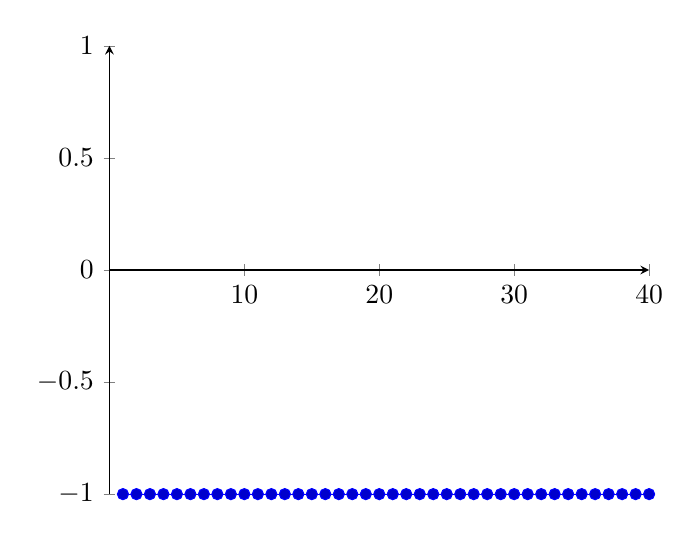
\begin{tikzpicture}
            \begin{axis}[
                ymin = -1,
                ymax = 1,
                xmin = 0,
                xmax = 40,
                axis x line=center,
                axis y line=left]
                \addplot coordinates {
                    (1,-1) (2,-1) (3,-1) (4,-1) (5,-1) (6,-1) (7,-1) (8,-1) (9,-1) (10,-1) (11,-1) (12,-1) (13,-1) (14,-1) (15,-1) (16,-1) (17,-1) (18,-1) (19,-1) (20,-1) (21,-1) (22,-1) (23,-1) (24,-1) (25,-1) (26,-1) (27,-1) (28,-1) (29,-1) (30,-1) (31,-1) (32,-1) (33,-1) (34,-1) (35,-1) (36,-1) (37,-1) (38,-1) (39,-1) (40,-1)
                };
                \end{axis}
            \end{tikzpicture}
            \caption{$c = -2, x_0 = 1$}
            \label{6.wyk1}
    \end{minipage}
    \quad
    \begin{minipage}{0.45\columnwidth}
        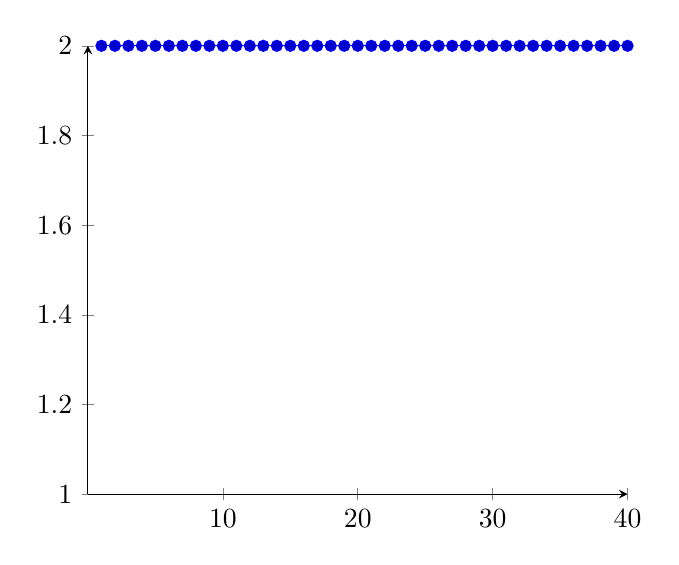
\begin{tikzpicture}
            \begin{axis}[
                ymin = 1,
                ymax = 2,
                xmin = 0,
                xmax = 40,
                axis x line=center,
                axis y line=left]
                \addplot coordinates {
                    (1,2) (2,2) (3,2) (4,2) (5,2) (6,2) (7,2) (8,2) (9,2) (10,2) (11,2) (12,2) (13,2) (14,2) (15,2) (16,2) (17,2) (18,2) (19,2) (20,2) (21,2) (22,2) (23,2) (24,2) (25,2) (26,2) (27,2) (28,2) (29,2) (30,2) (31,2) (32,2) (33,2) (34,2) (35,2) (36,2) (37,2) (38,2) (39,2) (40,2)
                };
                \end{axis}
            \end{tikzpicture}
            \caption{$c = -2, x_0 = 2$}
            \label{6.wyk2}
    \end{minipage}
\end{figure}

\begin{figure}[H]
    \centering
    \begin{minipage}{0.45\columnwidth}
        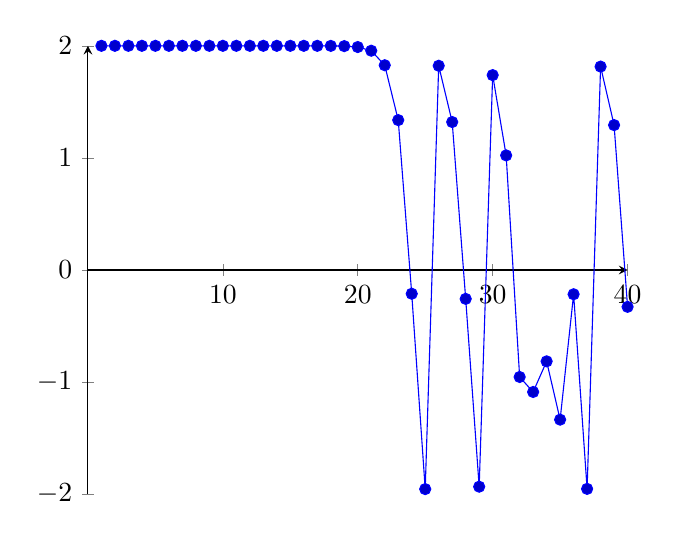
\begin{tikzpicture}
            \begin{axis}[
                ymin = -2,
                ymax = 2,
                xmin = 0,
                xmax = 40,
                axis x line=center,
                axis y line=left]
                \addplot coordinates {
                    (1,1.99999999999996) (2,1.9999999999998401) (3,1.9999999999993605) (4,1.999999999997442) (5,1.9999999999897682) (6,1.9999999999590727) (7,1.999999999836291) (8,1.9999999993451638) (9,1.9999999973806553) (10,1.999999989522621) (11,1.9999999580904841) (12,1.9999998323619383) (13,1.9999993294477814) (14,1.9999973177915749) (15,1.9999892711734937) (16,1.9999570848090826) (17,1.999828341078044) (18,1.9993133937789613) (19,1.9972540465439481) (20,1.9890237264361752) (21,1.9562153843260486) (22,1.82677862987391) (23,1.3371201625639997) (24,-0.21210967086482313) (25,-1.9550094875256163) (26,1.822062096315173) (27,1.319910282828443) (28,-0.2578368452837396) (29,-1.9335201612141288) (30,1.7385002138215109) (31,1.0223829934574389) (32,-0.9547330146890065) (33,-1.0884848706628412) (34,-0.8152006863380978) (35,-1.3354478409938944) (36,-0.21657906398474625) (37,-1.953093509043491) (38,1.8145742550678174) (39,1.2926797271549244) (40,-0.3289791230026702)
                };
                \end{axis}
            \end{tikzpicture}
            \caption{$c = -2, x_0 = 1.99999999999999$}
            \label{6.wyk3}
    \end{minipage}
    \quad
    \begin{minipage}{0.45\columnwidth}
        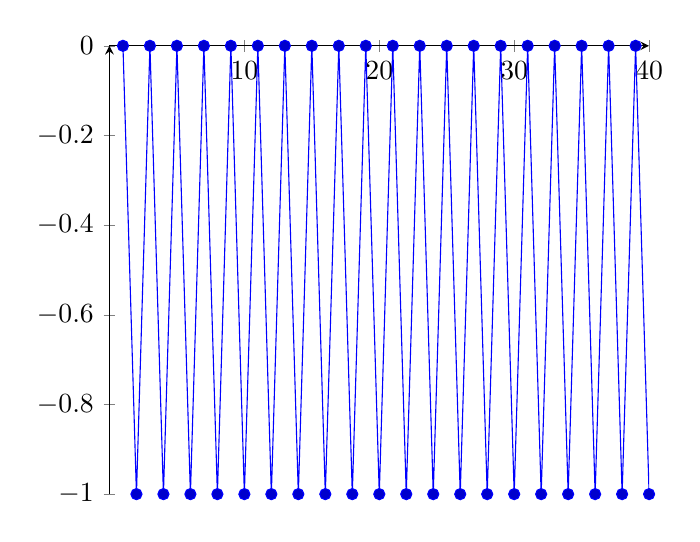
\begin{tikzpicture}
            \begin{axis}[
                ymin = -1,
                ymax = 0,
                xmin = 0,
                xmax = 40,
                axis x line=center,
                axis y line=left]
                \addplot coordinates {
                    (1,0) (2,-1) (3,0) (4,-1) (5,0) (6,-1) (7,0) (8,-1) (9,0) (10,-1) (11,0) (12,-1) (13,0) (14,-1) (15,0) (16,-1) (17,0) (18,-1) (19,0) (20,-1) (21,0) (22,-1) (23,0) (24,-1) (25,0) (26,-1) (27,0) (28,-1) (29,0) (30,-1) (31,0) (32,-1) (33,0) (34,-1) (35,0) (36,-1) (37,0) (38,-1) (39,0) (40,-1)
                };
                \end{axis}
            \end{tikzpicture}
            \caption{$c = -1, x_0 = 1$}
            \label{6.wyk4}
    \end{minipage}
\end{figure}

\begin{figure}[H]
    \centering
    \begin{minipage}{0.45\columnwidth}
        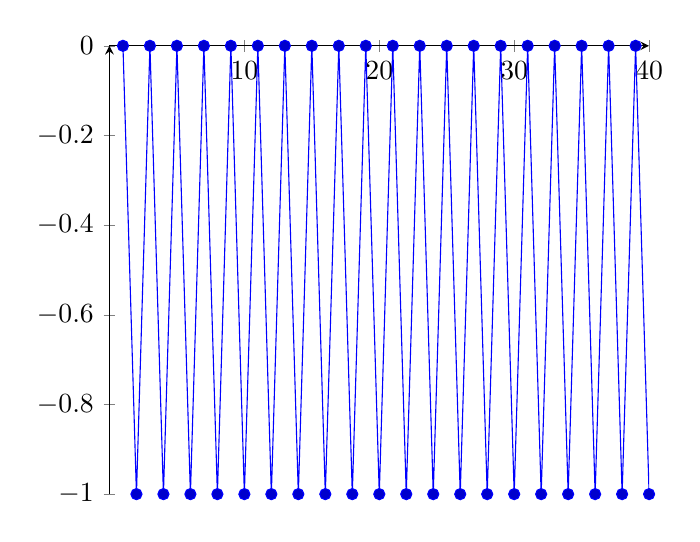
\begin{tikzpicture}
            \begin{axis}[
                ymin = -1,
                ymax = 0,
                xmin = 0,
                xmax = 40,
                axis x line=center,
                axis y line=left]
                \addplot coordinates {
                    (1,0) (2,-1) (3,0) (4,-1) (5,0) (6,-1) (7,0) (8,-1) (9,0) (10,-1) (11,0) (12,-1) (13,0) (14,-1) (15,0) (16,-1) (17,0) (18,-1) (19,0) (20,-1) (21,0) (22,-1) (23,0) (24,-1) (25,0) (26,-1) (27,0) (28,-1) (29,0) (30,-1) (31,0) (32,-1) (33,0) (34,-1) (35,0) (36,-1) (37,0) (38,-1) (39,0) (40,-1)
                };
                \end{axis}
            \end{tikzpicture}
            \caption{$c = -1, x_0 = -1$}
            \label{6.wyk5}
    \end{minipage}
    \quad
    \begin{minipage}{0.45\columnwidth}
        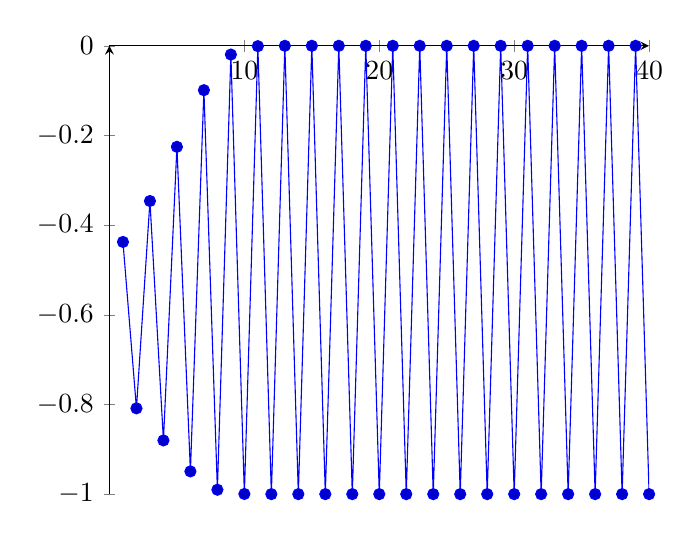
\begin{tikzpicture}
            \begin{axis}[
                ymin = -1,
                ymax = 0,
                xmin = 0,
                xmax = 40,
                axis x line=center,
                axis y line=left]
                \addplot coordinates {
                    (1,-0.4375) (2,-0.80859375) (3,-0.3461761474609375) (4,-0.8801620749291033) (5,-0.2253147218564956) (6,-0.9492332761147301) (7,-0.0989561875164966) (8,-0.9902076729521999) (9,-0.01948876442658909) (10,-0.999620188061125) (11,-0.0007594796206411569) (12,-0.9999994231907058) (13,-1.1536182557003727e-6) (14,-0.9999999999986692) (15,-2.6616486792363503e-12) (16,-1.0) (17,0.0) (18,-1.0) (19,0.0) (20,-1.0) (21,0.0) (22,-1.0) (23,0.0) (24,-1.0) (25,0.0) (26,-1.0) (27,0.0) (28,-1.0) (29,0.0) (30,-1.0) (31,0.0) (32,-1.0) (33,0.0) (34,-1.0) (35,0.0) (36,-1.0) (37,0.0) (38,-1.0) (39,0.0) (40,-1.0)
                };
                \end{axis}
            \end{tikzpicture}
            \caption{$c = -1, x_0 = 0.75$}
            \label{6.wyk6}
    \end{minipage}
\end{figure}

\begin{figure}[H]
    \centering
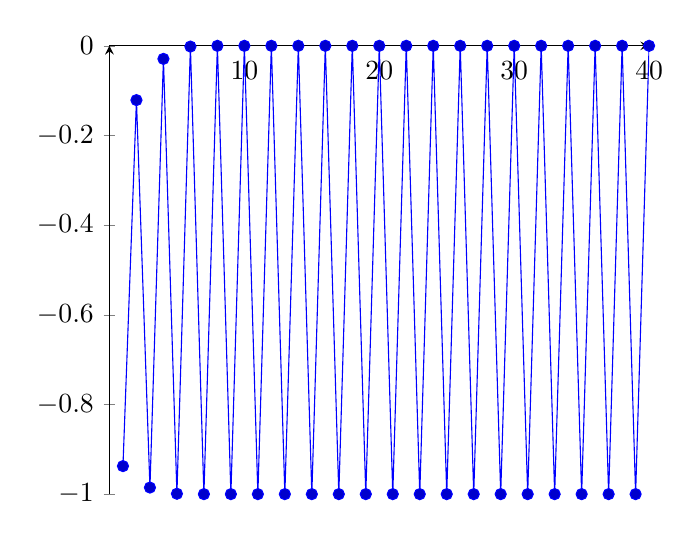
\begin{tikzpicture}
    \begin{axis}[
        ymin = -1,
        ymax = 0,
        xmin = 0,
        xmax = 40,
        axis x line=center,
        axis y line=left]
        \addplot coordinates {
            (1,-0.9375) (2,-0.12109375) (3,-0.9853363037109375) (4,-0.029112368589267135) (5,-0.9991524699951226) (6,-0.0016943417026455965) (7,-0.9999971292061947) (8,-5.741579369278327e-6) (9,-0.9999999999670343) (10,-6.593148249578462e-11) (11,-1.0) (12,0.0) (13,-1.0) (14,0.0) (15,-1.0) (16,0.0) (17,-1.0) (18,0.0) (19,-1.0) (20,0.0) (21,-1.0) (22,0.0) (23,-1.0) (24,0.0) (25,-1.0) (26,0.0) (27,-1.0) (28,0.0) (29,-1.0) (30,0.0) (31,-1.0) (32,0.0) (33,-1.0) (34,0.0) (35,-1.0) (36,0.0) (37,-1.0) (38,0.0) (39,-1.0) (40,0.0)
        };
        \end{axis}
    \end{tikzpicture}
\caption{$c = -1, x_0 = 0.25$}
\label{6.wyk7}
\end{figure}

W przypadkach \hyperref[6.wyk1]{1.} i \hyperref[6.wyk2]{2.} ciąg zachowuje się stabilnie, ale już w przypadku \hyperref[6.wyk3]{3.} można zauważyć niestabilność spowodowaną lekkim odchyleniem pierwszego wyrazu ciągu.

\noindent Punkty \hyperref[6.wyk4]{4.} i \hyperref[6.wyk5]{5.} są
przypadkami idealnego balansu funkcji migającej.

\noindent W przypadkach \hyperref[6.wyk6]{6.} i \hyperref[6.wyk7]{7.} mamy za to przejście od niestabilności do stabilnej funkcji migającej.

Powyższe eksperymenty po raz kolejny pokazują jak początkowo bardzo małe błędy mogą się kumulować i generować chaos numeryczny, który bardzo utrudnia analizę tego typów problemów.

\end{document}
